\documentclass{beamer}
%\usetheme{Madrid}
%\usetheme{Boadilla}
%\usetheme{default}
%\usetheme{Warsaw}
%\usetheme{Frankfurt}
\usetheme{Bologna}
%\usetheme{Bergen}
%\usetheme{Hannover}
%\usecolortheme{dolphin}
%\usetheme{Darmstadt}
%\setbeamertemplate{footline}[page number]
\setbeamercovered{transparent}
\setbeamercovered{invisible}
\setbeamertemplate{navigation symbols}{}
% To remove the navigation symbols from
% the bottom of slides

\usepackage[outline]{contour}
\usepackage{pgf}
\usepackage{graphicx}
\usepackage[english]{babel}
\usepackage[utf8]{inputenc}
\usepackage{listings}
\usepackage{xcolor}

\usepackage{url}
\usepackage{multicol}

%\usepackage[pdftex,bookmarks,colorlinks,%
%pdfauthor={Daniele Bellavista},%
%pdftitle={Shellcoding, and introduction},%
%pdftex]{hyperref}
%\usepackage{bm}  % For typesetting bold math (not \mathbold)

\definecolor{dkgreen}{rgb}{0,0.6,0}
\definecolor{gray}{rgb}{0.5,0.5,0.5}
\definecolor{mauve}{rgb}{0.58,0,0.82}

\newcommand{\ccode}{
	\lstset{ language=C, basicstyle=\footnotesize, numbers=none, numberstyle=\tiny\color{gray},backgroundcolor=\color{white},frame=single, captionpos=b, breaklines=true,title=\lstname, keywordstyle=\color{blue},commentstyle=\color{dkgreen}, showstringspaces=false, stringstyle=\color{mauve}, escapeinside={\%*}{*} }}

\newcommand{\acode}{
	\lstset{ language={[x86masm]Assembler}, basicstyle=\small, numbers=left, numberstyle=\tiny\color{gray},backgroundcolor=\color{white},frame=single, captionpos=b, breaklines=true,title=\lstname, keywordstyle=\color{blue},commentstyle=\color{dkgreen}, stringstyle=\color{mauve}, escapeinside={\%*}{*} }}

\newcommand{\acodenonu}{
	\lstset{ language={[x86masm]Assembler}, basicstyle=\small, numbers=none, backgroundcolor=\color{white},frame=single, captionpos=b, breaklines=true,title=\lstname, keywordstyle=\color{blue},commentstyle=\color{dkgreen}, stringstyle=\color{mauve}, escapeinside={\%*}{*} }}

\newcommand{\acodesmall}{
	\lstset{ language={[x86masm]Assembler}, basicstyle=\tiny, numbers=none, backgroundcolor=\color{white},frame=single, captionpos=b, breaklines=true,title=\lstname, keywordstyle=\color{blue},commentstyle=\color{dkgreen}, stringstyle=\color{mauve}, escapeinside={\%*}{*} }}

\title[Code and Data Injection]{Unexpected inputs: the danger of data and code injection}

\author[Daniele Bellavista]{Cesena Security Network and Applications}

\institute[CeSeNA]
{%
\emph{University of Bologna, Scuola di Ingegneria ed Architettura}\\
\emph{Ingegneria Informatica}
\emph{Scienze e Tecnologie dell'Informazione}
\emph{Ingegneria e Scienze Informatiche}
}

\logo{\pgfputat{\pgfxy(-1.5,7.8)}{\pgfbox[center,base]{%
  
\includegraphics[width=2.8cm]{./imgs/Cesena3.png}}}
}

\contourlength{1pt}
\contournumber{20}
\begin{document}

% CeSeNA, speakers presentation
{%
  \definecolor{myblue}{HTML}{B8C3E2}
	\setbeamertemplate{footline}{}
	\setbeamertemplate{navigation symbols}{}
  \setbeamertemplate{title page}{%
  \begin{picture}(0,0)
    \put(-11,-157){%
      
\includegraphics[height=\paperheight]{imgs/background2.jpg}
    }
    \put(110,-10){%
      
\includegraphics[height=1cm]{./imgs/Cesena2.png}
    }
    \put(25,-150){%
      \begin{minipage}[b][45mm][t]{100mm}
        \center
        \usebeamerfont{title}{\fontsize{0.8cm}{1em}\selectfont \textcolor{myblue}{%
          \contour{black}{Unexpected inputs:}
          \contour{black}{the danger of data and code injection}
        }\par}
      \end{minipage}
    }
  \end{picture}

  }
	\begin{frame}
	  \titlepage
	\end{frame}
}
\section{What's CeSeNA?}

\begin{frame}{Who are we?}

\begin{block}{Cesena Security and Network Applications}
  \begin{itemize}
    \item We like computer security and we want to share our knowledge.
    \item Founded by \emph{Marco Ramilli} in 2005.
    \item Rebuilt by \emph{Luca Mella} in 2009.
    \item Now it's an active group, managed by \emph{Alessandro Molari}, \emph{Luca
      Molari} and \emph{Giacomo Mantani}.
  \end{itemize}
\end{block}

\begin{block}{Why join CeSeNA?}
  \begin{itemize}
  \item To learn useful, cool stuff.
  \item To improve mental and social skills.
  \item To have (a lot of) fun!
  \end{itemize}
\end{block}
\end{frame}

\begin{frame}{Contact us!}

\begin{block}{Requirement to apply CeSeNA}
  \begin{itemize}
    \item Burning desire for knowledge.
    \item Passion for computer security.
    \item Be a geeky, techky person.
  \end{itemize}
\end{block}

\begin{block}{Where to find us}
  \begin{itemize}
  \item IRC: {\small \#cesena at irc.freenode.net}
  \item Website: {\small \url{https://cesena.ing2.unibo.it/}} (trust the certificate)
  \item Facebook: {\small \url{https://www.facebook.com/groups/105136176187559/} }
  \item G+: {\small \url{https://plus.google.com/communities/101402441314003721224}}
  \end{itemize}
\end{block}

\end{frame}


% CeSeNA, speakers presentation
{%
  \definecolor{myblue}{HTML}{B8C3E2}
	\setbeamertemplate{footline}{}
	\setbeamertemplate{navigation symbols}{}
  \setbeamertemplate{title page}{%
  \begin{picture}(0,0)
    \put(-11,-157){%
      
\includegraphics[height=\paperheight]{imgs/background3.jpg}
    }
    \put(110,-10){%
      
\includegraphics[height=1cm]{./imgs/Cesena2.png}
    }
    \put(25,-150){%
      \begin{minipage}[b][45mm][t]{100mm}
        \center
        \usebeamerfont{title}{\fontsize{0.8cm}{1em}\selectfont \textcolor{myblue}{%
          \contour{black}{INJECTION VULNERABILITY}
          %\contour{black}{the danger of data and code injection}
        }\par}
      \end{minipage}
    }
  \end{picture}

  }
	\begin{frame}
	  \titlepage
	\end{frame}
}
\section{Injection Vulnerability}

\begin{frame}{Injection: same old story}

\begin{block}{SQL injection}
  \begin{itemize}
    \item Introduced by sloppy \emph{(PHP)} programmers.
    \item One of the main vulnerability in 2000s.
    \item Still present and exploited!
  \end{itemize}
\end{block}

\begin{block}{Shellshock vulnerability}
  \begin{itemize}
    \item Discovered in 2014.
    \item Present since September 1989!
    \item In some scenarios, it permits remote code execution.
  \end{itemize}
\end{block}
\end{frame}

  \lstset{basicstyle=\small, frame=single, breaklines=true, escapeinside={\%*}{*} }
\begin{frame}[fragile]{SQLi example}
  \begin{itemize}
    \item \textbf{Scenario}: system containing secret stuff on the database, which can be accessed only by knowing their secret identifier.
    \item \textbf{Objective}: obtain all the secrets!
    \item SQL Query:
\ccode
\begin{lstlisting}
exec("SELECT * FROM Secrets WHERE SecId = " + secretId)
\end{lstlisting}
\pause
    \item If secretId is \textbf{1234567}
\begin{lstlisting}
exec("SELECT * FROM Secrets WHERE SecId = 1234567")
\end{lstlisting}
  \end{itemize}

\end{frame}
\begin{frame}[fragile]{SQLi example}

\ccode
\begin{itemize}
  \item Query:
  \begin{lstlisting}
  exec("SELECT * FROM Secrets WHERE ID = " + secretId)
  \end{lstlisting}
\pause
  \item Injection if secretId is \textbf{0 OR 1=1}:
\begin{lstlisting}
exec("SELECT * FROM Secrets WHERE ID = 0 OR 1=1")
\end{lstlisting}
\end{itemize}
\end{frame}

\begin{frame}[fragile]{A shellshock example}
  \begin{itemize}
    \item Request to a CGI page:
  \begin{lstlisting}
  GET /vulnerable.cgi
  User-Agent: Mozilla Firefox
  \end{lstlisting}
\pause
    \item Response:
  \begin{lstlisting}
  200 OK

  Hi, I'm not vulnerable!
  \end{lstlisting}
  \end{itemize}

\end{frame}

\begin{frame}[fragile]{A shellshock example}

  \begin{itemize}
    \item Request:
  \begin{lstlisting}
  GET /vulnerable.cgi
  User-Agent: () { ignored; }; echo The following sentence is false
  \end{lstlisting}
\pause
    \item Response:
  \begin{lstlisting}
  200 OK
  The following sentence is false

  Hi, I'm not vulnerable!
  \end{lstlisting}
  \end{itemize}
\end{frame}

\begin{frame}{Data and code are confused}
\begin{block}{Untrusted user-supplied inputs}
  \begin{itemize}
    \item Web form fields (yes, even hidden tags).
    \item HTTP fields.
    \item Shell parameters.
  \end{itemize}
\end{block}

\begin{block}{No difference between data and code}
  \begin{itemize}
    \item No data type.
    \item Semantic checks are performed only on the result.
  \end{itemize}
\end{block}
\end{frame}

\begin{frame}{Sanitization}
  \begin{itemize}
    \item \textbf{Whitelist} allowed character. Drop or escape the rest.
    \item \textbf{Type awareness:} parse integers, encode strings, etc..
    \item Use \textbf{framework or library functions} considered secure.
    \item Remember: \textbf{security isn't just a fix}.
  \end{itemize}
\end{frame}


% Exploitation
{%
  \definecolor{myblue}{HTML}{B8C3E2}
	\setbeamertemplate{footline}{}
	\setbeamertemplate{navigation symbols}{}
  \setbeamertemplate{title page}{%
  \begin{picture}(0,0)
    \put(-61,-157){%
      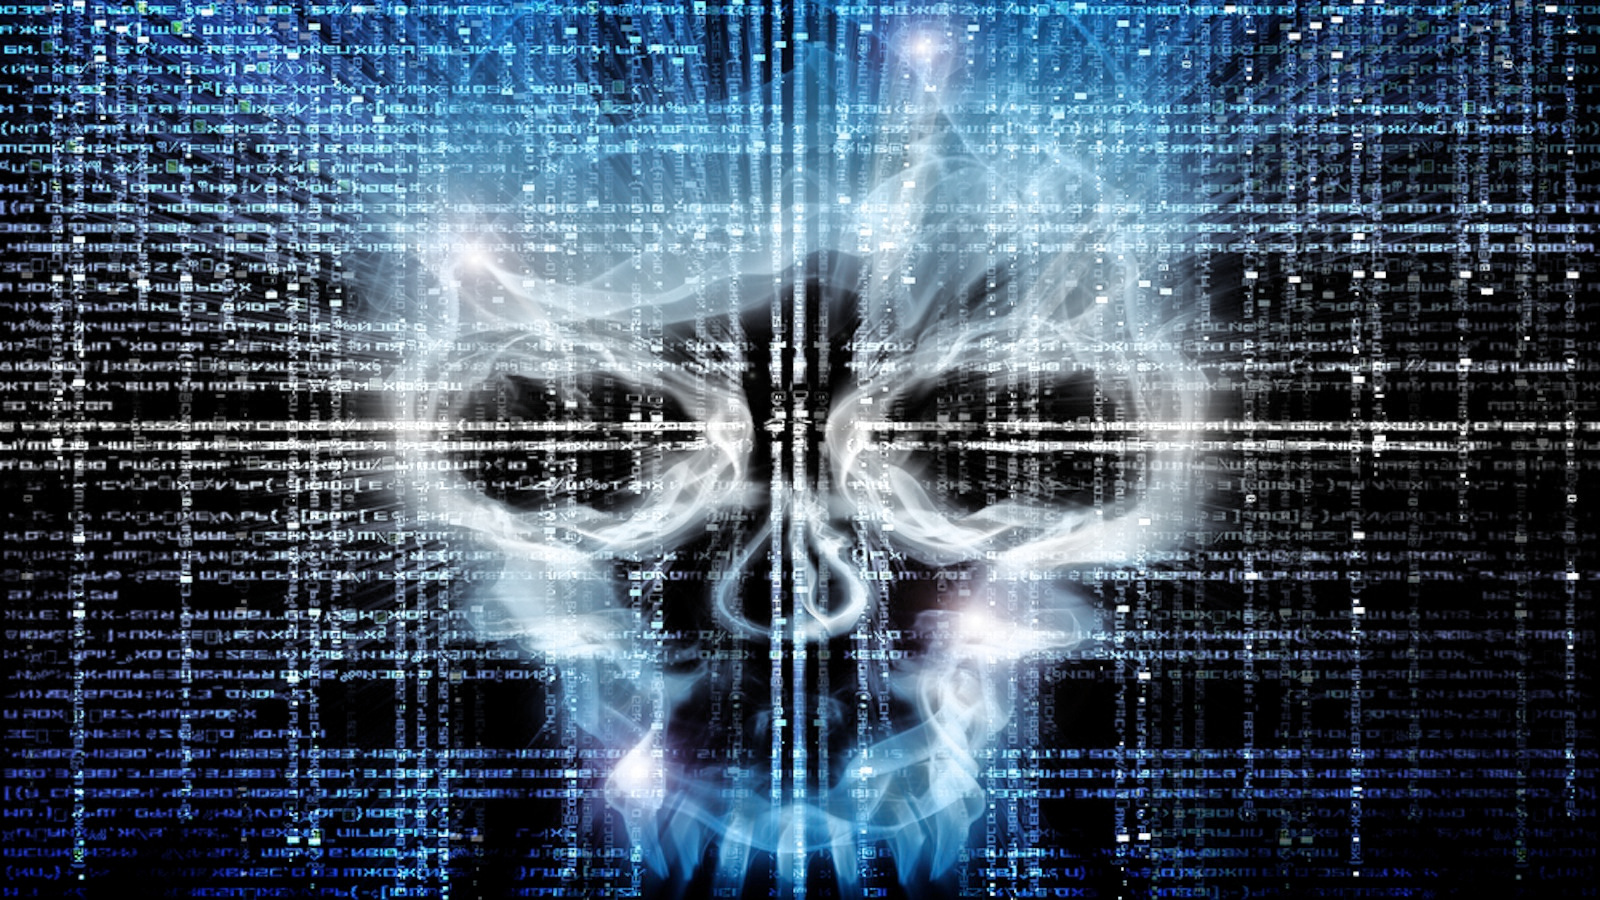
\includegraphics[height=\paperheight]{imgs/background4.jpg}
    }
    \put(110,-10){%
      
\includegraphics[height=1cm]{./imgs/Cesena2.png}
    }
    \put(25,-150){%
      \begin{minipage}[b][45mm][t]{100mm}
        \center
        \usebeamerfont{title}{\fontsize{0.8cm}{1em}\selectfont \textcolor{myblue}{%
          \contour{black}{EXPLOITATION}
          %\contour{black}{the danger of data and code injection}
        }\par}
      \end{minipage}
    }
  \end{picture}

  }
	\begin{frame}
	  \titlepage
	\end{frame}
}
\section{Exploiting Injection}

\begin{frame}[fragile]{Bad sanitization: quoting}
  \ccode
  \begin{itemize}
    \item Quoted SQL statement:
\begin{lstlisting}
"SELECT * FROM Secrets WHERE SecId = '" + secretId + "'"
\end{lstlisting}
\pause
    \item Previous secretId \textbf{= 0 OR 1=1} won't work!
\begin{lstlisting}
"SELECT * FROM Secrets WHERE SecId = '0 OR 1=1'
\end{lstlisting}
\pause
    \item So, just send secretId \textbf{= 0' OR '1'='1}
\begin{lstlisting}
"SELECT * FROM Secrets WHERE SecId = '0' OR '1'='1'
\end{lstlisting}
    \item Celebrate
  \end{itemize}
\end{frame}

\begin{frame}[fragile]{Bad sanitization: blind escaping}
  \ccode
  \begin{itemize}
    \item Quoted SQL statement:
\begin{lstlisting}
"SELECT * FROM Secrets WHERE SecId = '" +
                             escapeQuotes(secretId) + "'"
\end{lstlisting}
\pause
    \item The previous trick won't work: secretId = \textbf{0' OR '1'='1}
\begin{lstlisting}
"SELECT * FROM Secrets WHERE SecId = '0\' OR \'1\'=\'1'
\end{lstlisting}
\pause
    \item However, a similar query without quotes won't be protected!
\begin{lstlisting}
"SELECT * FROM Secrets WHERE SecId = " +
                                   escapeQuotes(secretId)
\end{lstlisting}
\pause
    \item Just try \textbf{0 OR 1=1}
\begin{lstlisting}
"SELECT * FROM Secrets WHERE SecId = 0 OR 1 = 1
\end{lstlisting}
  \end{itemize}
\end{frame}

\begin{frame}[fragile]{Bad sanitization: string replace}
  \ccode
  \begin{itemize}
    \item Smartest fix ever:
\begin{lstlisting}
"SELECT * FROM Secrets WHERE SecId = " +
                              replace(secretId, 'OR', '')
\end{lstlisting}
\pause
    \item If secretId \textbf{= 0 OR 1=1}
\begin{lstlisting}
"SELECT * FROM Secrets WHERE SecId = 0 1 = 1"
\end{lstlisting}
\pause
    \item What if, secretId \textbf{= 0 OORR 1=1}
\begin{lstlisting}
"SELECT * FROM Secrets WHERE SecId = 0 OR 1 = 1"
\end{lstlisting}
  \end{itemize}
\end{frame}


% Excercise
{%
  \definecolor{myblue}{HTML}{B8C3E2}
	\setbeamertemplate{footline}{}
	\setbeamertemplate{navigation symbols}{}
  \setbeamertemplate{title page}{%
  \begin{picture}(0,0)
    \put(-61,-157){%
      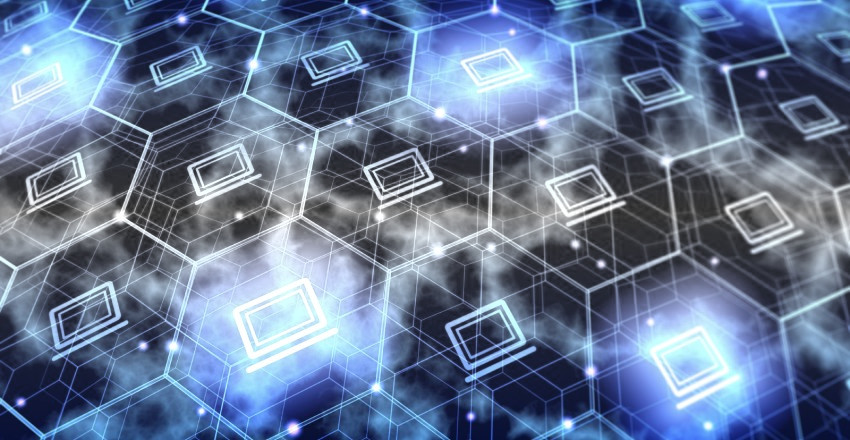
\includegraphics[height=\paperheight]{imgs/background5.jpg}
    }
    \put(110,-10){%
      
\includegraphics[height=1cm]{./imgs/Cesena2.png}
    }
    \put(25,-150){%
      \begin{minipage}[b][45mm][t]{100mm}
        \center
        \usebeamerfont{title}{\fontsize{0.8cm}{1em}\selectfont \textcolor{myblue}{%
          \contour{black}{IT'S YOUR TURN}
          %\contour{black}{the danger of data and code injection}
        }\par}
      \end{minipage}
    }
  \end{picture}

  }
	\begin{frame}
	  \titlepage
	\end{frame}
}
\section{Exercise}


\begin{frame}[fragile,allowframebreaks]{Tools}

\begin{block}{objdump - the linux disassembler}
		\begin{verbatim}
$ objdump -M intel -d <PROGNAME>
		\end{verbatim}
\end{block}
\framebreak		
\begin{block}{gdb - the linux debugger}
	\footnotesize
	\begin{verbatim}
$ gdb <PROGNAME>
(gdb) set disassembly-flavor intel   # we like intel sintax
(gdb) disassemble <SYMBOL-OR-ADDRESS>   # eg. disass main
(gdb) b * 0xdeadbeef			# breakpoint at address
(gdb) run <ARGS>	    # run the program
(gdb) stepi         # step into
(gdb) nexti         # step over
(gdb) finish	        # run until ret
(gdb) i r           # info registers
(gdb) i b           # info breakpoints
(gdb) x/20i	$eip	    # print 20 instr starting from EIP
(gdb) x/20w	$esp	    # 'w' WORD, 's' STRING, 'd' 
                       DECIMAL, 'b' BYTE
(gdb) display/<X-EXPR>	# like x/ but launched 
                           at every command
	\end{verbatim}
	\normalsize
\end{block}
\end{frame}

\begin{frame}[fragile,allowframebreaks]{Exercise}
	Exercises source available at \url{http://goo.gl/WupDs}\\
	Some exercises need to connect via ssh to cesena.ing2.unibo.it\\
	 as pwn at port 7357 to test your solution.\\
	(ssh pwn@cesena.ing2.unibo.it -p 7357)\\
	\begin{figure}
		\centering
		
\includegraphics[height=.4\textheight]{imgs/qrcode.png}
		\caption{Exercises source}
		\label{fig:qrcode}
	\end{figure}
\framebreak
	\begin{block}{Warming up}
		\emph{auth}\\
		Just a basic overflow.\\
		Don't look too far, it's just next to you.
	\end{block}
\framebreak
	\begin{block}{Function pointer overwrite}
		\emph{nameless}\\
		Hey! A function pointer!\\
		Yes, we probably need \emph{gdb}
	\end{block}
\framebreak
	\begin{block}{Return OverWrite Easy}
		\emph{rowe}\\
		We are getting serious\\
		You'll have to OverWrite the return address!
	\end{block}
\framebreak
	\begin{block}{Return OverWrite Hard}
		\emph{rowh}\\
		Just like the previuos, but can you also prepare the data on the stack?
	\end{block}
\framebreak
	\begin{block}{Notes program}
		\emph{note}\\
		Sample notes program, ./note reads the notes, ./note "my note" adds a note\\
		You'll need a shellcode.
	\end{block}
\end{frame}


{%
  \definecolor{myblue}{HTML}{B8C3E2}
	\setbeamertemplate{footline}{}
	\setbeamertemplate{navigation symbols}{}
  \setbeamertemplate{title page}{%
  \begin{picture}(0,0)
    \put(-61,-157){%
      
\includegraphics[height=\paperheight]{imgs/background6.jpg}
    }
    \put(110,-30){%
      
\includegraphics[height=1cm]{./imgs/Cesena2.png}
    }
    %\put(25,-150){%
      %\begin{minipage}[b][45mm][t]{100mm}
        %\center
        %\usebeamerfont{title}{\fontsize{0.8cm}{1em}\selectfont \textcolor{myblue}{%
          %\contour{black}{IT'S YOUR TURN}
          %%\contour{black}{the danger of data and code injection}
        %}\par}
      %\end{minipage}
    %}
  \end{picture}

  }
	\begin{frame}
	  \titlepage
	\end{frame}
}
%\section{References}
\begin{frame}[allowframebreaks]{References}
	\bibliographystyle{plain}
	\nocite{reference}
	\nocite{*}
	\bibliography{references}{}
\end{frame}

\end{document}
